\scanpage{133}
\margin{provient du \uline{complexe \unsure{idélique}} $J$ par \unsure{multiplication} par $n$}
\figure{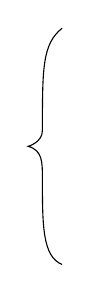
\begin{tikzpicture}[x=1cm,y=1cm]
\draw (0.25,3) .. controls (0,2.8) and (0,2.5) .. (0,1.7) .. controls (0,1.55) and (-0.18,1.5) .. (-0.18,1.5) .. controls (0,1.45) and (0,1.3) .. (0,1.1) .. controls (0,0.5) and (0,0.1) .. (0.25,0);
\end{tikzpicture}}
\diagram{\begin{array}{c|c}
\mu_n,\quad(n,p)=1 & \mathbb Z/n\mathbb Z\qquad(n,p)=1\\[5pt]
\mu_n,\quad {}_nJ,\quad\mathbb Z/n\mathbb Z & \mathbb Z/n\mathbb Z=\mu_n\otimes\mu_n^\vee,\quad {}_nJ\otimes\mu_n^\vee,\quad\mu_n^\vee\\[8pt]\hline
\mu_p & \mathbb Z/p\mathbb Z\\[5pt]
\mu_p,\quad {}_pJ,\quad\mathbb Z/p\mathbb Z & \mathbb Z/p\mathbb Z,\quad {}_{(1-F)}H^1(C,\underline O_C)^{\unsure{F}},\quad H^1(C,\underline O_C)_{(1-F)}=0\\[8pt]\hline
\alpha_p & \alpha_p\\[5pt]
\alpha_p,\quad {}_FH^1(C,\underline O_C),\quad H^1(C,\underline O_C)_F & \text{''}\\[8pt]\hline\hline
G_m & \mathbb Z\\[5pt]
\bigl[G_m,\quad\underline{\operatorname{Pic}}^{\unsure{0|\bullet}}_{C/k},\quad0, & \mathbb Z,\quad0,\quad H^1(C,\mathbb Q/\mathbb Z)=\operatorname{Hom}(T(J),\mathbb Q/\mathbb Z),\quad H^2(C,\mathbb Q/\mathbb Z)\simeq\underset{(n,p)=1}{\varinjlim}\mu_n^\vee,\quad0,\bigr]\
\end{array}}
\margin{\unsure{autodualité} des \unsure{S.} \unsure{gr. d'ordre fini} de la \deleted{\unsure{Jacobienne}}}
\margin{$\Delta({}_pJ)\simeq H^1(C,\underline O_C)^F$\par
$\phantom{\Delta({}_pJ)}\qquad\Vert$\par
$\phantom{\Delta({}_pJ)}\quad(H^1(C,\mathbb Z/p\mathbb Z))$\par
i.e. $\pi_1(C)\otimes\mathbb Z/p\mathbb Z\simeq{}_pJ$\par
[autodualité de la Jacobienne \unsure{pour} $\unsure{V,F|p}$]}
[provient du \uline{complexe adélique} $A$ par application du \deleted{\unsure{p}} \inserted{Frobenius}]
\margin{Dualité \unsure{élémentaire} de $H^1(C,\underline O_C)_F$ et ${}_FH^1(C,\underline O_C)$ provient de l'autodual. d'ordre infinitésimal de la Jacobienne, \unsure{du plus gd sous-groupe de} $A$ [\unsure{ou} ${}_pA$] isomorphe à un $\alpha_p^n$, est dual au \unsure{plus gd quotient} de ${}_pA$ ayant la \unsure{même} propriété, cette dualité provenant d'une dualité des algèbres de Lie correspondantes.}

Pour $G=G_m$, le th. de dualité s'écrit \deleted{\unsure{pour tout groupe}}
\[
H^*(C,\unsure{\sigma|\tau})\simeq
\underline{\operatorname{Ext}}^*\bigl(\underbrace{Rf_*(G_m)}_{\substack{\text{complexe}\\\text{\unsure{idélique}}}}(-1),\unsure{\sigma|\tau}\bigr)
\Longleftarrow\underline{\operatorname{Ext}}^{\unsure{p+q}}(R^{-q}f_*(G_m),\unsure{\sigma|\tau})
\]
et on se ramène au cas \uline{géométrique}, et $\unsure{\sigma|\tau}=\mathbb Q/\mathbb Z$.
\[
H^*(C,\mathbb Q/\mathbb Z)\simeq\underline{\operatorname{Ext}}^*(Rf_*(G_m)(1),\unsure{\sigma|\tau})
\Longleftarrow\underline{\operatorname{Ext}}^{\unsure{i-j}}(R^{-j}f_*(G_m),\mathbb Q/\mathbb Z).
\]
et on calcule :
\[
H^0(C,\mathbb Q/\mathbb Z)\simeq\mathbb Q/\mathbb Z,\qquad
H^1(C,\mathbb Q/\mathbb Z)\simeq\operatorname{Ext}^1(J^{\unsure{0|\bullet}},\mathbb Q/\mathbb Z),\qquad
H^2(C,\mathbb Q/\mathbb Z)\simeq\varinjlim\mu_n^\vee
\]
\inserted{$\operatorname{Ext}^1(J^0,\mathbb Q/\mathbb Z),\quad\Vert$}
\margin{autodualité de la Jacobienne}
\figure{\begin{tikzpicture}[x=1cm,y=1cm]
\draw[<-] (0,0) -- (2.3,0.1);
\draw (2.4,0.2) .. controls (2.6,0.7) and (3.2,0.8) .. (3.6,1.1);
\draw (-3,-0.4) -- (7,-0.25);
\end{tikzpicture}}
\mspage{132}

